\chapter{Logam Transisi dan Kompleks Koordinasi}\label{ch:b2:coordination-complexes}

Pada tahun 1893 seorang kimiawan berusia dua puluh enam tahun, Alfred
Werner, berusaha menjelaskan sebuah teka-teki. Kobalt(III) klorida membentuk
empat senyawa dengan amonia, \ce{CoCl3.6NH3}, \ce{CoCl3.5NH3}, dan dua dengan
rumus \ce{CoCl3.4NH3}, yang satu hijau dan yang lain ungu. Perak nitrat
langsung mengendapkan ketiga klorida senyawa pertama, dua klorida senyawa
kedua, dan hanya satu klorida dari masing-masing dua senyawa terakhir.
Jawaban Werner --- enam gugus yang tertahan di sekeliling logam pada
sudut-sudut sebuah oktahedron, sisanya di luar --- meletakkan dasar kimia
koordinasi. Bab ini memperluas kompleks-kompleks jilid Tahun 1 ke
geometrinya, isomer-isomernya, nama-namanya, dan sebuah perhitungan
elektron yang meramalkan karbonil logam mana yang ada.

\begin{recall}
Jilid Tahun 1: kompleks, atom pusat, ligan, ligan polidentat, kelat, tetapan
pembentukan, bilangan koordinasi; konfigurasi elektron ion-ion logam
transisi (elektron $n$s lepas lebih dahulu); asam dan basa Lewis, ikatan
datif; VSEPR; bilangan oksidasi; enansiomer. \Cref{ch:b2:atomic-orbitals}:
orbital-orbital d dan urutan tingkat 4s dan 3d.
\end{recall}

\begin{omfigure}
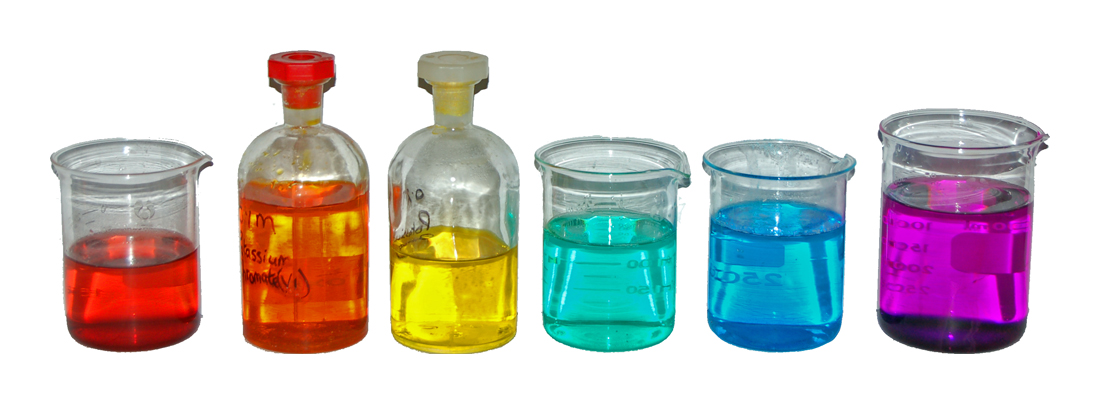
\includegraphics[width=0.8\linewidth]{images/book3/tm-solutions.jpg}

{\small Larutan berair senyawa-senyawa logam transisi: dari kiri ke kanan,
kobalt(II) nitrat, kalium dikromat, kalium kromat, nikel(II) klorida,
tembaga(II) sulfat, dan kalium permanganat. Warna larutan kobalt, nikel, dan
tembaga berasal dari kompleks akuanya. (Foto: Benjah-bmm27, domain publik,
Wikimedia Commons.)}
\end{omfigure}

\section{Blok d}

\begin{definition}[Unsur transisi]\label{def:b2:coordination-complexes:transition-element}
Yang disebut \emph{unsur transisi}\index{unsur transisi} adalah unsur yang
atomnya, atau salah satu ionnya yang lazim, mempunyai subkulit d yang terisi
sebagian. Ion unsur semacam itu dengan $n$ elektron dalam orbital-orbital d-nya
mempunyai \emph{konfigurasi $d^n$}\index{konfigurasi dn@konfigurasi $d^n$}.
\end{definition}

\begin{proposition}[Menghitung elektron d]\label{prop:b2:coordination-complexes:dn}
Ion logam transisi $\mathrm M^{m+}$ dari golongan bernomor $g$ (3 sampai 12)
mempunyai konfigurasi $d^n$ dengan $n = g - m$.
\end{proposition}

\begin{proof}
Atom netralnya mempunyai $g$ elektron di luar gas mulia sebelumnya, dalam
orbital $n$s dan $(n - 1)$d. Dalam ion-ionnya, orbital-orbital d terletak di
bawah orbital s (\cref{ex:b2:atomic-orbitals:iron}): semua $g - m$ elektron
valensi yang tersisa adalah elektron d.
\end{proof}

Sebagai contoh, \ce{Fe^2+} (golongan 8) adalah $d^6$, \ce{Cu^2+} (golongan 11) $d^9$,
\ce{Co^3+} (golongan 9) $d^6$, \ce{Pt^2+} (golongan 10) $d^8$.

\section{Ligan}

\begin{definition}[Dentisitas]\label{def:b2:coordination-complexes:denticity}
Yang disebut \emph{dentisitas}\index{dentisitas} sebuah ligan adalah jumlah
atomnya yang terikat pada atom pusat yang sama. Sebuah \emph{ligan
monodentat}\index{ligan monodentat} terikat melalui satu atom (\ce{H2O},
\ce{NH3}, \ce{Cl-}, \ce{CO}), sebuah \emph{ligan
bidentat}\index{ligan bidentat} melalui dua (etana-1,2-diamina, ditulis en;
ion etanadioat, ox). Sebuah \emph{ligan jembatan}\index{ligan jembatan}
terikat pada dua atom logam sekaligus. Sebuah \emph{ligan
ambidentat}\index{ligan ambidentat} dapat terikat melalui salah satu dari
dua atom yang berbeda, seperti ion nitrit (melalui N atau O) atau tiosianat
(melalui S atau N).
\end{definition}

\begin{definition}[Bola koordinasi]\label{def:b2:coordination-complexes:coordination-sphere}
Yang disebut \emph{bola koordinasi}\index{bola koordinasi} sebuah kompleks
adalah himpunan atom pusat dan ligan-ligan yang terikat padanya, yang
dituliskan di dalam kurung siku; ion-ion di luar kurung adalah ion lawan,
yang tidak terikat pada logam.
\end{definition}

\begin{omfigure}
\setchemfig{atom sep=2.2em}
\chemfig{M*5(-H_2N-CH_2-CH_2-NH_2-)}
\qquad
\chemfig{M*5(-O-(=O)-(=O)-O-)}
\qquad
\chemfig{N(-[:120]CH_2COO^{-})(-[:240]CH_2COO^{-})-CH_2-CH_2-N(-[:60]CH_2COO^{-})(-[:-60]CH_2COO^{-})}

\medskip
{\small Ligan-ligan pengelat. Kiri: etana-1,2-diamina (en), bidentat melalui
kedua nitrogennya. Tengah: ion etanadioat (ox), bidentat melalui dua
oksigen. Kanan: anion edta, yang membungkus ion logam dengan kedua
nitrogennya dan keempat oksigen karboksilatnya (heksadentat).}
\end{omfigure}

\section{Bilangan koordinasi dan geometri}

Dua, empat, dan enam adalah bilangan koordinasi yang paling lazim. Perak(I)
dan emas(I) membentuk kompleks linear (\ce{[Ag(NH3)2]+}); empat ligan
membentuk tetrahedron (\ce{[CoCl4]^2-}, \ce{[Zn(NH3)4]^2+}) atau bujur
sangkar (\ce{[PtCl4]^2-}, \ce{[Ni(CN)4]^2-}); lima, bipiramida trigonal
(\ce{Fe(CO)5}); enam, yang sejauh ini paling sering, oktahedron.

\begin{omfigure}
\begin{tikzpicture}[font=\small]
  \node[omligand] at (-0.8,0) {}; \node[omligand] at (0.8,0) {};
  \draw[thick, black!70] (-0.8,0) -- (0.8,0); \node[ommetal] at (0,0) {};
  \node at (0,-1.5) {linear, 2};
  \pic at (3,0) {omtetrahedron}; \node at (3,-1.5) {tetrahedral, 4};
  \pic at (6,0) {omsquareplanar}; \node at (6,-1.5) {bujur sangkar, 4};
  \pic at (9,0) {omtbp}; \node[align=center] at (9,-1.65) {bipiramida\\ trigonal, 5};
  \pic at (12,0) {omoctahedron}; \node at (12,-1.5) {oktahedral, 6};
\end{tikzpicture}

{\small Geometri-geometri koordinasi yang lazim (logam jingga, ligan abu-abu;
ikatan putus-putus mengarah ke belakang halaman).}
\end{omfigure}

VSEPR, yang menempatkan pasangan-pasangan elektron atom pusat sejauh mungkin
satu sama lain, gagal di sini: ion $d^8$ seperti \ce{Pt^2+} membawa empat
pasang elektron d dan empat ligan, namun kompleks-kompleksnya berbentuk bujur
sangkar, bukan tetrahedral atau oktahedral. Elektron-elektron d bukanlah
pasangan-pasangan terlokalisasi yang mendorong ligan: energinya bergantung
pada geometri dengan cara yang dihitung dalam bab berikutnya.

\begin{proposition}[$d^8$ bujur sangkar]\label{prop:b2:coordination-complexes:square-planar}
Kompleks berkoordinasi empat dari ion-ion $d^8$ deret transisi kedua dan
ketiga (\ce{Pd^2+}, \ce{Pt^2+}, \ce{Au^3+}) berbentuk bujur sangkar planar.
\end{proposition}

\admitted

Penjelasannya, yaitu pemisahan tingkat-tingkat d oleh ligan, diberikan pada
\cref{ch:b2:ligand-field}.

\section{Isomer}

\begin{definition}[Isomer kompleks]\label{def:b2:coordination-complexes:isomers}
Dalam kompleks oktahedral $\mathrm{MA_3B_3}$, \emph{isomer fac}\index{isomer fac}
mempunyai ketiga ligan B pada satu muka oktahedron, sedangkan \emph{isomer
mer}\index{isomer mer} pada sebuah meridian (tiga posisi dalam satu bidang
yang melalui logam). \emph{Isomer ikatan}\index{isomer ikatan} berbeda dalam
atom yang dipakai \omterm{def:b2:coordination-complexes:denticity}{ligan ambidentat} untuk terikat. \emph{Isomer
ionisasi}\index{isomer ionisasi} saling menukar sebuah ligan dengan ion
lawan, sehingga menghasilkan ion-ion yang berbeda dalam larutan.
\end{definition}

\begin{proposition}[Menghitung isomer oktahedral]\label{prop:b2:coordination-complexes:isomer-count}
Dalam oktahedron, $\mathrm{MA_4B_2}$ mempunyai dua isomer (cis dan trans), $\mathrm{MA_3B_3}$ dua
(fac dan mer), dan $\mathrm M(\mathrm{AA})_3$, dengan tiga \omterm{def:b2:coordination-complexes:denticity}{ligan bidentat},
dua enansiomer, $\Delta$ dan $\Lambda$.
\end{proposition}

\begin{proof}
Dalam oktahedron, setiap dua posisi bertetangga (cis, $90^\circ$) atau
berseberangan (trans, $180^\circ$): dua susunan untuk kedua ligan B. Untuk
tiga ligan B, entah tidak ada dua yang trans (ketiganya menempati satu muka:
fac) atau tepat satu pasang yang trans (yang ketiga cis terhadap keduanya:
mer); tiga posisi yang saling trans tidak ada. Untuk
$\mathrm M(\mathrm{AA})_3$, setiap kelat merentang dua posisi cis; ketiga
kelat melilit sumbu lipat tiga seperti bilah-bilah baling-baling, berputar
searah atau berlawanan arah jarum jam jika dilihat sepanjang sumbu itu: dua
bayangan cermin, yang tidak dapat ditumpukkan karena kompleks itu tidak
mempunyai bidang cermin.
\end{proof}

\begin{omfigure}
\begin{tikzpicture}[font=\scriptsize]
  \pic (a) at (0,0) {omoctahedron};
  \node[omligand, fill=omDef!70] at (a-L1) {}; \node[omligand, fill=omDef!70] at (a-L3) {};
  \node at (0,-1.5) {\small cis-$\mathrm{MA_4B_2}$};
  \pic (b) at (3,0) {omoctahedron};
  \node[omligand, fill=omDef!70] at (b-L1) {}; \node[omligand, fill=omDef!70] at (b-L2) {};
  \node at (3,-1.5) {\small trans-$\mathrm{MA_4B_2}$};
  \pic (c) at (6.5,0) {omoctahedron};
  \node[omligand, fill=omThm!70] at (c-L1) {}; \node[omligand, fill=omThm!70] at (c-L3) {}; \node[omligand, fill=omThm!70] at (c-L5) {};
  \node at (6.5,-1.5) {\small fac-$\mathrm{MA_3B_3}$};
  \pic (d) at (9.5,0) {omoctahedron};
  \node[omligand, fill=omThm!70] at (d-L1) {}; \node[omligand, fill=omThm!70] at (d-L2) {}; \node[omligand, fill=omThm!70] at (d-L3) {};
  \node at (9.5,-1.5) {\small mer-$\mathrm{MA_3B_3}$};
\end{tikzpicture}

\medskip
\begin{tikzpicture}[font=\scriptsize]
  \foreach \xs/\s/\lab in {0/1/{$\Delta$}, 4.5/-1/{$\Lambda$}} {
    \begin{scope}[xshift=\xs cm, xscale=\s]
      \draw[black!30] (0,0) circle (1.2);
      \foreach \a in {90, 210, 330} {
        \coordinate (p) at (\a:1.1); \coordinate (q) at (\a+70:0.55);
        \draw[very thick, omDef] (\a:1.1) .. controls (\a+30:1.25) and (\a+60:0.9) .. (\a+75:0.55);
        \node[omligand] at (\a:1.1) {}; \node[omligand] at (\a+75:0.55) {};
      }
      \node[ommetal] at (0,0) {};
    \end{scope}
    \node at (\xs,-1.6) {\small \lab};
  }
  \draw[densely dashed] (2.25,-1.3) -- (2.25,1.3);
  \node[anchor=south] at (2.25,1.3) {cermin};
\end{tikzpicture}

{\small Atas: isomer cis dan trans $\mathrm{MA_4B_2}$ (ligan B biru), \omterm{def:b2:coordination-complexes:isomers}{isomer fac}
dan mer $\mathrm{MA_3B_3}$ (B merah). Bawah: kedua enansiomer sebuah tris-kelat
seperti \ce{[Co(en)3]^3+}, dilihat sepanjang sumbu lipat tiga, skematis:
setiap kelat (busur biru) menghubungkan sebuah posisi atas dan sebuah
posisi bawah, dan ketiganya berputar ke satu arah ($\Delta$) atau ke arah
yang lain ($\Lambda$).}
\end{omfigure}

\section{Nama dan jumlah elektron}

\begin{method}[Menamai kompleks]\label{met:b2:coordination-complexes:naming}
\begin{enumerate}
  \item Dalam rumus, tuliskan \omterm{def:b2:coordination-complexes:coordination-sphere}{bola koordinasi} di dalam kurung siku, logamnya
        lebih dahulu, lalu ligan-ligannya; muatan kompleks di luar kurung.
  \item Dalam nama, urutkan ligan-ligan menurut abjad dengan awalan pengali
        (di-, tri-, tetra-; bis-, tris- untuk nama ligan yang majemuk): ligan
        anionik berakhiran -o (klorido, sianido, oksido, hidroksido), ligan
        netral mempertahankan namanya (akua, amin, karbonil).
  \item Kemudian logamnya, yang namanya diberi akhiran seperti pada ferat,
        kuprat, dan kobaltat jika kompleksnya anion, dan bilangan oksidasinya
        dalam angka Romawi.
  \item Kation dinamai sebelum anion: \ce{[Co(NH3)6]Cl3} adalah
        heksaaminkobalt(III) klorida, \ce{K4[Fe(CN)6]} kalium
        heksasianidoferat(II).
\end{enumerate}
\end{method}

\begin{definition}[Jumlah elektron]\label{def:b2:coordination-complexes:electron-count}
Yang disebut \emph{jumlah elektron valensi}\index{jumlah elektron valensi}
sebuah kompleks adalah banyaknya elektron d ion logam ditambah elektron
yang diberikan oleh ligan-ligan (dua untuk setiap pasangan donor). Yang
disebut \emph{aturan 18 elektron}\index{aturan 18 elektron} menyatakan bahwa
kompleks-kompleks stabil dari logam berbilangan oksidasi rendah dengan
ligan akseptor $\pi$ yang berikatan kuat seperti \ce{CO} cenderung mempunyai
18 elektron valensi.
\end{definition}

\begin{definition}[Hapisitas]\label{def:b2:coordination-complexes:hapticity}
Yang disebut \emph{hapisitas}\index{hapisitas} sebuah ligan adalah jumlah
atomnya yang terikat pada logam melalui satu sistem $\pi$ yang
berkesinambungan; hapisitas ditulis $\eta^n$: etena yang terikat melalui
ikatan $\pi$-nya adalah $\eta^2$, cincin siklopentadienil yang terikat melalui
kelima karbonnya $\eta^5$.
\end{definition}

\begin{method}[Menghitung elektron]\label{met:b2:coordination-complexes:electron-count}
\begin{enumerate}
  \item Berikan muatan kepada ligan-ligan sebagai spesies berkulit tertutup
        (\ce{Cl-}, \ce{H-}, \ce{C5H5-}; \ce{CO}, \ce{PR3}, \ce{NH3} netral) dan
        simpulkan bilangan oksidasi logamnya.
  \item Hitunglah elektron d logam itu, $n = g - m$.
  \item Tambahkan dua elektron per pasangan donor: satu per \omterm{def:b2:coordination-complexes:denticity}{ligan monodentat},
        enam untuk $\eta^5$-\ce{C5H5-}, enam untuk $\eta^6$-benzena, dua untuk
        $\eta^2$-alkena.
  \item Ikatan logam--logam dihitung satu elektron untuk masing-masing logam.
\end{enumerate}
\end{method}

\begin{proposition}[Karbonil logam]\label{prop:b2:coordination-complexes:eighteen}
Karbonil-karbonil biner yang stabil dari deret transisi pertama, \ce{Cr(CO)6},
\ce{Fe(CO)5}, \ce{Ni(CO)4}, dan \ce{Mn2(CO)10}, semuanya mempunyai 18 elektron
valensi per atom logam.
\end{proposition}

\begin{proof}
Kromium(0), $d^6$, dengan enam CO: $6 + 12 = 18$. Besi(0), $d^8$, lima CO: $8 + 10 = 18$.
Nikel(0), $d^{10}$, empat CO: $10 + 8 = 18$. Mangan(0), $d^7$, lima CO dan
satu ikatan Mn--Mn: $7 + 10 + 1 = 18$; \ce{Mn(CO)5} monomerik, dengan 17,
tidak ada sebagai senyawa yang stabil, dan berpasangan. Alasan mengapa 18
lebih disukai --- sembilan orbital valensi logam, yang semua \omterm{def:b2:diatomic-mos:bonding}{orbital ikatan}
atau nonikatannya terisi --- diberikan pada \cref{ch:b2:ligand-field}.
\end{proof}

Ferosena, \ce{Fe(\eta^5-C5H5)2}, menahan sebuah ion besi(II) ($d^6$) di antara
dua anion siklopentadienil, yang masing-masing memberikan enam elektron:
$6 + 12 = 18$. Aturan ini gagal untuk sebagian besar kompleks berbilangan
oksidasi tinggi dan untuk banyak kompleks dengan ligan lemah:
\ce{[Ti(H2O)6]^3+} mempunyai 13 elektron, \ce{[Cu(H2O)6]^2+} 21.

\begin{history}[Werner dan oktahedron]
\begin{minipage}[t]{0.22\linewidth}
\vspace{0pt}
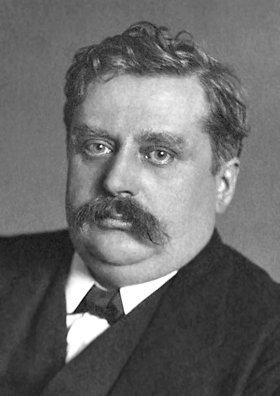
\includegraphics[width=\linewidth]{images/book3/werner.jpg}
\end{minipage}\hfill
\begin{minipage}[t]{0.74\linewidth}
\vspace{0pt}
Alfred Werner mengusulkan pada tahun 1893 bahwa sebuah logam mempunyai,
selain valensinya, bilangan koordinasi berupa gugus-gugus yang tertahan
langsung di sekelilingnya, dan bahwa kobalt(III) menahan enam gugus pada
sudut-sudut sebuah oktahedron. Ia lalu meramalkan berapa isomer yang
seharusnya dimiliki setiap rumus dan menghabiskan dua puluh tahun untuk
membuatnya; pada tahun 1911 ia memisahkan sebuah kompleks kobalt menjadi
kedua enansiomernya, yang membuktikan bahwa kekiralan tidak memerlukan atom
karbon. Ia menerima Hadiah Nobel Kimia pada tahun 1913. (Potret, Les Prix
Nobel, 1914, domain publik, Wikimedia Commons.)
\end{minipage}
\end{history}

\section{Latihan}

\begin{exercise}[$\star$]\label{exo:b2:coordination-complexes:1}
Tuliskan konfigurasi $d^n$ \ce{Ti^3+}, \ce{V^3+}, \ce{Cr^3+}, \ce{Mn^2+},
\ce{Fe^3+}, \ce{Co^2+}, \ce{Ni^2+}, dan \ce{Zn^2+}.
\end{exercise}

\begin{exercise}[$\star$]\label{exo:b2:coordination-complexes:2}
Tentukan \omterm{def:b2:coordination-complexes:denticity}{dentisitas} air, etana-1,2-diamina, ion etanadioat, edta, dan ion
tiosianat, dan sebutkan mana yang ambidentat.
\end{exercise}

\begin{exercise}[$\star$]\label{exo:b2:coordination-complexes:3}
Namailah \ce{[Cu(NH3)4]SO4}, \ce{K3[Fe(CN)6]}, \ce{[CoCl2(NH3)4]Cl}, dan
\ce{[Ni(CO)4]}.
\end{exercise}

\begin{exercise}[$\star$]\label{exo:b2:coordination-complexes:4}
Ramalkan geometri \ce{[Ag(NH3)2]+}, \ce{[CoCl4]^2-}, \ce{[PtCl4]^2-}, dan
\ce{[Fe(H2O)6]^2+}.
\end{exercise}

\begin{exercise}[$\star\star$]\label{exo:b2:coordination-complexes:5}
Berapa isomer yang dimiliki \ce{[PtCl2(NH3)2]} bujur sangkar planar?
Gambarlah isomer-isomer itu. (Salah satunya, sisplatin, adalah obat
antikanker.)
\end{exercise}

\begin{exercise}[$\star\star$]\label{exo:b2:coordination-complexes:6}
Hitunglah elektron valensi \ce{Cr(CO)6}, \ce{Fe(CO)5}, \ce{Ni(CO)4},
\ce{V(CO)6}, dan \ce{Mn2(CO)10}. Senyawa manakah yang melanggar aturan itu,
dan bagaimana perilakunya?
\end{exercise}

\begin{exercise}[$\star\star$]\label{exo:b2:coordination-complexes:7}
Hitunglah elektron valensi ferosena dan kobaltosena \ce{Co(C5H5)2}. Senyawa
manakah yang mudah teroksidasi, dan menjadi apa?
\end{exercise}

\begin{exercise}[$\star\star$]\label{exo:b2:coordination-complexes:8}
Kompleks nikel(II) dengan edta mempunyai $\log_{10}K = 20.5$, jauh di atas
kompleks-kompleks yang nikelnya terikat pada enam donor nitrogen atau oksigen
yang terpisah. Jelaskan efek kelat ini dari segi jumlah partikel yang
dilepaskan ketika kelat itu menggantikan enam molekul air.
% ledger: logb:Ni-edta
\end{exercise}

\begin{exercise}[$\star\star$]\label{exo:b2:coordination-complexes:9}
Gambarlah kedua \omterm{def:b2:coordination-complexes:isomers}{isomer ikatan} \ce{[Co(NO2)(NH3)5]^2+}.
\end{exercise}

\begin{exercise}[$\star\star\star$]\label{exo:b2:coordination-complexes:10}
Berapa stereoisomer yang dimiliki \ce{[CoCl2(en)2]+}? Manakah yang kiral?
\end{exercise}

\begin{exercise}[$\star\star\star$]\label{exo:b2:coordination-complexes:11}
Untuk $\mathrm{MA_4B_2}$, hitunglah isomer-isomer yang diramalkan oleh
heksagon planar dan oleh prisma trigonal dengan enam ligan, dan jelaskan
bagaimana jumlah isomer yang ditemukan menentukan pilihan di antara
geometri-geometri itu.
\end{exercise}

\begin{exercise}[$\star\star\star$]\label{exo:b2:coordination-complexes:12}
Hitunglah elektron valensi \ce{[RhCl(PPh3)3]} dan \ce{[IrH(CO)(PPh3)3]}
(\ce{PPh3} donor dua elektron, \ce{H-} sebagai hidrida). Senyawa manakah
yang dapat mengikat dua ligan lagi?
\end{exercise}

\section{Soal: Kobalt Amin Werner}

\begin{problem}[{Soal akhir pekan --- empat amin kobalt(III) klorida dan
klorida yang dilepaskannya, rumusnya dengan kurung siku, kedua isomer
tetraamin dan apa yang dibuktikannya tentang geometri, serta aktivitas
optik sebuah tris-kelat}]
\label{pb:b2:coordination-complexes:1}
Data: empat senyawa A \ce{CoCl3.6NH3} (kuning jingga), B \ce{CoCl3.5NH3}
(lembayung), C dan D \ce{CoCl3.4NH3} (hijau dan ungu). Dengan perak nitrat
berlebih, satu mol A mengendapkan 3 mol \ce{AgCl}, B 2 mol, C dan D
masing-masing 1 mol. Konduktivitas molar menunjukkan 4, 3, 2, dan 2 ion per
satuan rumus.

\medskip
\noindent\textbf{Bagian I --- Klorida dan ion.}
\begin{enumerate}
  \item Klorida manakah yang langsung bereaksi dengan ion perak?
  \item Berapa klorida yang terikat pada kobalt dalam setiap senyawa?
  \item Cocokkan jumlah ion dengan konduktivitasnya.
  \item Berapa bilangan oksidasi kobalt dalam keempat senyawa itu?
  \item Apa konfigurasi $d^n$-nya?
  \item Berapa jumlah total ligan yang ditahan kobalt dalam setiap senyawa?
\end{enumerate}

\medskip
\noindent\textbf{Bagian II --- Rumus dan nama.}
\begin{enumerate}[resume]
  \item Tuliskan A, B, C, dan D dengan kurung siku.
  \item Namailah A dan B.
  \item Namailah kation C dan D.
  \item Isomer jenis apakah C dan D?
  \item Akan menjadi apakah senyawa \ce{CoCl3.3NH3}, dan berapa ion yang akan
        dihasilkannya?
  \item Berapa isomer yang akan dimiliki senyawa itu dalam oktahedron?
\end{enumerate}

\medskip
\noindent\textbf{Bagian III --- Geometri.}
\begin{enumerate}[resume]
  \item Gambarlah \ce{[CoCl2(NH3)4]+} cis dan trans dalam oktahedron.
  \item Hitunglah isomer-isomer \ce{[CoCl2(NH3)4]+} yang diramalkan untuk
        enam ligan pada sudut-sudut heksagon planar.
  \item Hitunglah isomer yang diramalkan untuk prisma trigonal.
  \item Werner tidak pernah menemukan lebih dari dua. Apa yang dibuktikannya?
  \item Apakah bukti itu lengkap? Apa arti isomer ketiga seandainya ada?
  \item Manakah di antara C dan D yang cis, jika diketahui bahwa isomer cis
        dapat diubah menjadi kelat dengan etanadioat sedangkan isomer trans
        tidak dapat?
\end{enumerate}

\medskip
\noindent\textbf{Bagian IV --- Aktivitas optik.}
\begin{enumerate}[resume]
  \item Gambarlah \ce{[Co(en)3]^3+}.
  \item Apakah kation itu mempunyai bidang cermin? Pusat inversi?
  \item Berapa stereoisomer yang dimilikinya?
  \item Apa yang dibuktikan oleh pemisahan kation semacam itu menjadi
        enansiomer-enansiomernya?
  \item Apakah \ce{[CoCl2(en)2]+} kiral dalam bentuk cis-nya? Dalam bentuk
        trans-nya?
  \item Mengapa pemisahan oleh Werner atas sebuah kompleks yang sama sekali
        tidak mengandung karbon itu penting?
  \item Nyatakan jumlah isomer \ce{[CoCl2(NH3)4]+} yang diramalkan oleh
        oktahedron, dan oleh heksagon planar serta prisma trigonal.
\end{enumerate}
\end{problem}
